% Diese Zeile bitte -nicht- aendern.
\documentclass[course=erap]{aspdoc}

%%%%%%%%%%%%%%%%%%%%%%%%%%%%%%%%%
%% TODO: Ersetzen Sie in den folgenden Zeilen die entsprechenden -Texte-
%% mit den richtigen Werten.
\newcommand{\theGroup}{103} % Beispiel: 42
\newcommand{\theNumber}{A300} % Beispiel: A123
\author{Ngoc Kim Ngan Nguyen \and Yll Kryeziu \and Keihan Pakseresht}
\date{Sommersemester 2023} % Beispiel: Wintersemester 2019/20
%%%%%%%%%%%%%%%%%%%%%%%%%%%%%%%%%

% Diese Zeile bitte -nicht- aendern.
\title{Gruppe \theGroup{} -- Abgabe zu Aufgabe \theNumber}

\begin{document}
\maketitle

%======================= 1. Einleitung =========================================
\section{Einleitung}
Der \emph{Fast Inverse Square Root} Algorithmus, auch bekannt unter dem Namen \emph{Quake} Algorithmus ist ein berühmter Algorithmus aus dem Bereich der Computergrafik. Erstmalige Berühmtheit erlangte er im Jahre 2005 als der Source-Code des 3D First-Person-Shooters \emph{Quake III: Arena} veröffentlicht wurde. Der Algorithmus nähert sich auf Basis mathematischer Berechnungen mit einer hohen Genauigkeit an den Kehrwert der Wurzel einer 32-Bit Floating-Point Zahl an und macht sich dabei das IEEE 754 Format und die newtonsche Annäherung zunutze. \par
Die Motivation für diesen Algorithmus liegt hinter prozessorintensiven Echtzeitberechnungen für Ein- und Ausfallswinkel und Reflektionen im Zusammenhang mit Simulationen von Licht und Schatten im dreidimensionalen Raum. In diesem Zusammenhang war es oftmals nötig, Vektoren zu normalisieren beziehungsweise ihren zugehörigen Normalvektor \(\hat{v}\) zu berechnen \cite{Robertson}.
\[\hat{v} = \frac{\vec v}{\lVert \vec v \rVert}\]
Der Betrag des Vektors kann über den Satz des Pythagoras berechnet werden und entspricht der euklidschen Norm.
\[{\lVert \vec v \rVert}\ = \sqrt{(v_{1})^{2}+(v_{2})^{2}+(v_{3})^{2}}\]
Zu Zeiten von \emph{Quake III: Arena} war dieser Algorithmus um einiges schneller als die herkömmliche Wurzelfunktion und Division, deren Geschwindigkeit für die Anforderungen des Videospiels nicht ausreichte. Der geringe Präzisionsverlust war dabei vernachlässigbar. \par
In dieser Ausarbeitung wird der \emph{Fast Inverse Square Root} Algorithmus hinsichtlich seiner Implementierung, mathematischen Grundlagen und Performanz analysiert und mit äquivalenten Alternativen verglichen. Im Zusammenhang wird ein Programm implementiert, dass den \emph{Fast Inverse Square Root} Algorithmus, beziehungsweise eine SIMD-optimierte Version davon, auf aus dem Terminal oder aus einer Datei eingelesene Float- und Double-Zahlen anwendet und somit die Kehrwerte ihrer Wurzeln berechnet und ausgibt. \par
Da die Aufgabenstellung keine genauere Angaben darüber macht, ob und wie die Werte aus der Eingabedatei und dem Terminal kombiniert werden, wird im Rahmenprogramm lediglich eine der beiden Eingabemethoden erlaubt. Die zusätzliche Option \emph{-t} startet die Ausführung der Tests und Benchmarks, die einige Minuten andauern und \emph{.csv} Dateien mit Messwerten im Ordner \emph{benchmark\_outputs} generieren.

%====================== 2. Lösungsansatz =======================================
%
\section{Lösungsansatz}
%--------------------------------2.1--------------------------------------------
\subsection{Relevante Hintergründe}
Das IEEE 754 Format und das Newtonverfahren sind wesentlich für die Funktionsweise des Algorithmus, weshalb die beiden Konzepte kurz erläutert werden, bevor diskutiert wird, wieso die Gleichung \(y = \frac{1}{\sqrt{x}} \approx \text{MagicNumber} - (x >> 1)\) aus dem Algorithmus gelten kann.\par
\textbf{IEEE 754} ist eine Standarddarstellung für Gleitkommazahlen. In diesem Format lassen sich Gleitkommazahlen durch drei Komponenten darstellen: Sign \(S\), Exponent \(E\) und Mantisse \(M\). Eine Gleitkommazahl wird als Kombination der Binärdarstellung der drei Komponenten dargestellt. Siehe Tabelle 1 für die Verteilung der Bits.
\begin{table}[ht]
\centering
\begin{tabular}{lcccl}
\cline{2-4}
\multicolumn{1}{c|}{}                                 & \multicolumn{1}{c|}{\textbf{Sign}}  & \multicolumn{1}{c|}{\textbf{Exponent}} & \multicolumn{1}{c|}{\textbf{Mantisse}} &  \\ \cline{2-4}
\multicolumn{1}{l|}{Float (32 Bit single precision)}  & \multicolumn{1}{c|}{1 Bit} & \multicolumn{1}{c|}{8 Bits}   & \multicolumn{1}{c|}{23 Bits}  &  \\ \cline{2-4}
\multicolumn{1}{l|}{Double (64 Bit double precision)} & \multicolumn{1}{c|}{1 Bit} & \multicolumn{1}{c|}{11 Bits}  & \multicolumn{1}{c|}{52 Bits}  &  \\ \cline{2-4}
                                                      & \multicolumn{1}{l}{}       & \multicolumn{1}{l}{}          & \multicolumn{1}{l}{}          & 
\end{tabular}
\caption{Bitzahl der Komponenten je nach Datentyp.}
\label{tab:captionIEEE}
\end{table}
Der Wert einer im IEEE 754 Format gespeicherten Zahl ergibt sich aus Gleichung 1, indem man die Komponenten als numerische Werte betrachtet.
\begin{equation}
    x = (-1)^S*\left(1+\frac{M}{2^N}\right)*2^{E-b}
\end{equation}
Um den numerischen Wert der Mantisse zu erhalten werden die Mantissen Bits als reale Zahl betrachtet und durch \(2^N\) dividiert, wobei \(N\) die Anzahl der Bits in der Mantisse ist. Da die Mantisse immer mit 1 beginnt, werden nur die Nachkommastellen in den Mantissenbits abzuspeichern, folglich hat die Mantisse einen Wertebereich von [0, 1). Der Exponent wird als vorzeichenlose Binärzahl gespeichert. Durch das Abziehen der sogenannten Bias \(b\) können negative Exponenten ohne das Zweierkomplement gespeichert werden. Die Bias beträgt für Floats \(127\) und für Doubles \(1023\) \cite{ieee754}. Mit Gleichung 2 erhält man die Integerdarstellung einer Zahl im IEEE 754 Format, wovon später Gebrauch gemacht wird.
\begin{equation}
    x_{\text{bits}} = 2^N * \left(E + \frac{M}{2^N}\right)
\end{equation}
Das Rahmenprogramm der Implementierung verhindert die Eingabe von negativen Zahlen und 0, somit ist das Sign Bit immer 0 und muss in weiteren Berechnungen nicht beachtet werden. \par
Das \textbf{Newton-Raphson-Verfahren} ist ein mathematischer Algorithmus zur numerischen Annäherung von Nullstellen einer Funktion. Es basiert auf der Verwendung von Tangenten an den Funktionsgraphen, um schrittweise bessere Schätzungen für die Nullstelle zu finden. Das Verfahren konvergiert in der Regel schnell gegen die genaue Lösung, wenn eine gute Startschätzung vorhanden ist. Ausgehend von einer vorhergehenden Nullstelle \(x_n\) ergibt sich die nächste, präzisere Nullstelle aus
\begin{equation}
    x_{n+1} = x_n * \frac{f(x_n)}{f'(x_n)} 
\end{equation}
wobei $f'(x_n)$ die Ableitung von $f(x_n)$ nach $x_n$ ist. Diese Iteration wird so oft ausgeführt, bis die gewünschte Genauigkeit erreicht ist \cite{newton}.
%--------------------------------2.2--------------------------------------------
\subsection{Funktionsweise des Algorithmus}
Der originale Sourcecode des Algorithmus kann auf dem Github-Account von id-Software gefunden werden \cite{qsqrt}. Zentral für den Algorithmus ist folgende Codezeile, wobei \lstinline{i} die Integerdarstellung der Gleitkommazahl ist, von der der Kehrwert der Wurzel berechnet wird: \lstinline{i  = 0x5F3759DF - (i >> 1);}. Nach der Zuweisung ist \lstinline{i} eine sehr guter Ausgangspunkt für anschließende Annäherung durch das Newtonverfahren. Im Folgenden wird der Grund dafür erläutert. Aus Gleichung 1 folgt durch Vereinfachung mit dem Logarithmus folgende Gleichung:
\begin{align}
    x &= \left(1+\frac{M}{2^{23}}\right)*2^{E-127} \nonumber\\
    \Rightarrow \log_2(x) &= \log_2\left(1+\frac{M}{2^{23}}\right)+ E-127
\end{align}
Weiteres gilt für eine Zahl $c$ in $[0, 1)$: $\log_2(1+c) \approx c + \sigma$, wobei $\sigma$ ein freier Parameter ist, der zum Optimieren der Annäherung verwendet wird \cite{McEniry}. Da die Mantisse nur in diesem Bereich liegt, gilt Gleichung 5. Hierbei ist die Integerdarstellung von $x$ nützlich.
\begin{align}
    \log_2(x) &= E+\frac{M}{2^{23}} -127 + \sigma \nonumber\\
    \Rightarrow \log_2(x) &= \frac{2^{23}*\left(E+\frac{M}{2^{23}}\right)}{2^{23}} -127 + \sigma \nonumber \\
    \Rightarrow \log_2(x) &= \frac{x_{\text{bits}}}{2^{23}} - 127 + \sigma
\end{align}
Gleichung 5 wird nun in die eigentliche Berechnung eingesetzt. Ebenfalls wird die Integerdarstellung von \(y\) benutzt.
\begin{align}
    y &= \frac{1}{\sqrt{x}} \nonumber\\
    \log_2(y) &= -\frac{1}{2}*\log_2(x) \nonumber\\
    \frac{y_{\text{bits}}}{2^{23}} - 127 + \sigma &= -\frac{1}{2}*\left(\frac{x_{\text{bits}}}{2^{23}} - 127 + \sigma \right) \nonumber\\
    y_{\text{bits}} &= \underbrace{\frac{3}{2}*2^{23}*(127-\sigma)}_{\text{MagicNumber}} - \underbrace{x_{\text{bits}}*\frac{1}{2}}_{\text{\lstinline{(i >> 1)}}}
\end{align}
Demnach korrespondiert \(\frac{3}{2}*2^{23}*(127-\sigma)\) zur konstanten MagicNumber, die der Fehlerkorrektur durch das Shiften dient, und \(x_{\text{bits}}*\frac{1}{2}\) zum Bitshift nach rechts, der einer Halbierung der Integerdarstellung von \(x\) entspricht. Die Berechnung einer geeigneten MagicNumber, sodass die hohe Genauigkeit des Algorithmus sichergestellt ist, erfolgt in Kapitel 2.3. \par
Nachdem ein angemessener Ausgangspunkt gefunden wurde, wird das Ergebnis nun mit der newton'schen Annäherung verbessert. Dies geschieht durch die Codezeile:
\begin{center}
    \lstinline{y = y * (threehalfs - (x2 * y * y));}
\end{center}
Durch geeignete Umformungen wird der Zusammenhang zum Newton-Raphson-Verfahren ersichtlich. Es ist $y = \frac{1}{\sqrt{x}}$ zu bestimmen. Diese Aufgabe ist äquivalent dazu, die Nullstellen $y$ der folgenden Funktion zu finden:
\begin{equation*}
    f(y) = \frac{1}{y^2} - x
\end{equation*}
%Das erhaltene \(x\) muss möglichst mit dem \(x_{input}\) übereinstimmen, auf das die Funktion angewendet wird, das heißt, deren Differenz sollte idealerweise 0 sein. Demnach erfolgt mit der Funktion dieser Differenz und dem newton'schen Verfahren eine Annäherung zum exakten Ergebnis \(y\).
Ist eine gute Startschätzung gegeben, erhält man die nächste, präzisere Nullstelle Einsetzen in die Formel des Newton-Raphson-Verfahrens:
\begin{equation}
    y_{n+1} = y_n - \frac{f(y_n)}{f'(y_n)} 
    = y_n - \frac{\frac{1}{y_n^2} - x}{\frac{-2}{y_n^3}} 
    = y_n + \frac{y_n - xy_n^3}{2}
    = y_n * \left(\frac{3}{2} - \frac{x}{2}*y_n^2\right)
\end{equation}
Mit den Zuweisungen \lstinline{float threehalfs = 1.5f} und \lstinline{float x2 = x * 0.5f} aus dem originalen Sourcecode ist die Funktion der Codezeile und schlussendlich des gesamten Algorithmus geklärt.

%--------------------------------2.2---------------------------------------------
% Das von uns entwickelte Verfahren zur Berechnung der Magic Number
\subsection{Die MagicNumber}
In dieser Implementierung wird ein \emph{Brute-Force-}Ansatz benutzt, um die MagicNumber zu bestimmen. Er basiert auf den Beobachtungen von Narayanareddy \cite{preetham}. Es werden verschiedene Werte der MagicNumber für die Implementierung für Floats und Doubles getestet und herausgefunden, welche Zahl den geringsten maximalen relativen Fehler über alle Zahle gibt. Aus Kapitel 2.2 Gleichung 6 ist die Form der MagicNumber (ab jetzt mit $R$ genannt) schon bekannt:
\begin{equation}
    R = \frac{3}{2} * 2^{23} * (127 - \sigma)
\end{equation}
wobei $\sigma$ ein freier Parameter ist, der zum Optimieren der Annäherung $\log_2(1 + c) = c + \sigma$ verwendet wird.\par
%-----
\subsubsection{Eingrenzungen des Suchfelds}
% 0x5F30_0000
Da $\log_2(1 + c) \ge c$ für alle Werte von $c$ in [0, 1) gilt und die Gleichheit nur an beiden Grenzen passiert, ist es leicht zu erkennen dass $\sigma > 0$ im Vergleich mit $\sigma \le 0$ eine bessere Annäherung gibt.\par
Aus (8) folgt $R = \frac{3}{2} * 2^{23} * 127 - \frac{3}{2} * 2^{23} * \sigma
< \frac{3}{2} * 2^{23} * 127 = \text{0x5F400000}$. Darüber hinaus ist $\sigma$ ein sehr kleiner Wert, was bedeutet, dass das Suchfeld zunächst zwischen \textbf{0x5F300000} und \textbf{0x5F400000} eingegrenzt werden kann.\par
% Optimiere Mantisse
Anstatt alle möglichen Werte von $x_{\text{bits}}$, was der Integerdarstellungen aller Floats entspricht, zu prüfen, können die meisten Exponentenbits zunächst ignoriert werden, um die Anzahl der Testfälle zu reduzieren. Die Genauigkeit des Verfahrens bleibt größtenteils bestehen, da $\sigma$ nur in der Näherungsformel der Mantisse $\log_2(1 + \frac{M}{2^{23}}) = \frac{M}{2^{23}} + \sigma$ vorkommt. Lediglich das niedrigstwertige Bit $E_0$ der Exponentenbits spielt eine große Rolle, weil es durch den Rechtsshift \lstinline{i >> 1} in das Mantissenfeld des Ergebnisses fällt. Hierbei müssen also $2^{24}$ Tests für jede MagicNumber stattfinden.\par
% Minimiere Suchfeld der Mantisse
Zuletzt können noch die Testwerte der Mantisse der MagicNumber $R$ eingeschränkt werden. Anstatt alle Werte der MagicNumber einzeln durchzuprobieren, können die Testwerte Ziffer für Ziffer vom höchstwertigen Bit zum niedrigstwertigen Bit eingegrenzt werden. Dies geschieht durch eine Inkrementierung in Schritten von \textbf{0x10000}, dann \textbf{0x1000} und so weiter, bis alle Ziffern gefunden sind. Auf diese Weise werden statt eine Millionen nur etwa 160 Werte geprüft.
%-----
\subsubsection{Ergebnis und Güte der bestimmten MagicNumber}
Nach Implementierung eines C-Programms nach dem oben beschriebenen Verfahren ist \boldmath $R = \textbf{0x5F375A87}$ \unboldmath die gefundene MagicNumber für Floats, die über alle Floats einen maximalen relativen Fehler von 0.1751350679\% hat. Das Verfahren zur Bestimmung der Genauigkeit wird in Kapitel 3 behandelt, aber es sei erwähnt, dass dies die Genaugigkeit nach einer Newtoniteraion ist. Die von uns berechnete MagicNumber ist sehr nah an Lomont's und Robertson's MagicNumber von \textbf{0x5F375A86}, die einen etwas geringeren maximalen relativen Fehler von 0.1751341630\% liefert. Es ist ersichtlich, dass die Zahl etwas schlechter in Genauigkeit ist. Dies liegt vor allem daran, dass die Exponenten von $x_\text{bits}$ im Laufe des Verfahrens ignoriert werden und somit eine Abweichung des maximalen relativen Fehlers von jedem Wert der MagicNumber entsteht.
%------
\subsubsection{Erweiterung auf Doubles mit 64 Bit}
Analog wird hier ebenfalls ein \emph{Brute-Force-}Ansatz mit Eingrenzungen des Suchbereichs benutzt. Allerdings muss es aus praktischen Gründen mehrere Einschränkungen der Testwerte geben.\par
\textbf{Erste Startschätzung:}
Da $R = \text{0x5F375A87}$ einen geringen maximalen relativen Fehler liefert, kann festgestellt werden, dass $\sigma$, gegeben durch die Gleichung
\begin{equation}
    \frac{3}{2} * 2^{23} * (127 - \sigma) = \text{0x5F375A87}
\end{equation}
eine hinreichend gute Approximation für $\log_2(1 + c) = c + \sigma$ bezüglich der \emph{Fast Inverse Square Root} Funktion anbietet. Aus (9) folgt der Wert von $\sigma$:
\begin{equation}
    \sigma = 127 - \frac{R}{\frac{3}{2} * 2^{23}} \approx 0.0450332165
\end{equation}
Die Gleichung (8) zur Bestimmung der MagicNumber lässt sich auf Double Zahlen erweitern, wobei $N$ die Anzahl der Bits der Mantisse und $b$ die Bias seien:
\begin{equation*}
    R_d = \frac{3}{2} * 2^{N} * (b - \sigma) 
    = \frac{3}{2} * 2^{52} * (1023 - \sigma)
\end{equation*}
Eine Substitution von $\sigma$ durch Gleichung (10) ergibt folgendes Ergebnis:
\begin{align}
    R_d &= \frac{3}{2} * 2^{52} * \left(1023 - \left(127 - \frac{R}{\frac{3}{2} * 2^{23}}\right)\right) \nonumber \\
    &= (1023 - 127) * \frac{3}{2} * 2^{52} + R * 2^{52 - 23}
    = \text{0x5FE6EB50E0000000}
\end{align}
Es ist zu beobachten, dass die unteren 29 Bits von $R_d$ Nullen sind. Dies entspricht genau die Differenz zwischen der Anzahl der Mantissenbits von Floats und Doubles. Analog zu dem oben beschriebenen Verfahren können die Testwerte der MagicNumber Ziffer für Ziffer eingegrenzt werden. Es werden zunächst die Werte um $2^{32} = \textbf{0x100000000}$ kleiner oder größer von $R_d$ getestet. Hierbei sind ungefähr 256 Werte von $R_d$ zu testen.\par
%Robertsons: 0x5fe6eb50c7b537a9 - 0.17511836712204020827
%Lomonts:    0x5fe6ec85e7de30da
%Berechnet:  0x5fe6eb50c632a7a2 (20 bit Mantisse getestet)
%            0x5fe6eb50c70e666e (22 bit Mantisse getestet)
%            0x5fe6eb50c77c4635 (23 bit Mantisse getestet)
%            0x5fe6eb50c7b33600 (24 bit Mantisse getestet) 0.17511836687917892164
%            0x5fe6eb50c7b33600 (25 bit Mantisse getestet) 0.175118
%            0x5fe6eb50c7b33600 (26 bit Mantisse getestet) 0.175118
% Initial value => 0.175119
% 5fe6eb50e0000000 - 0x5FE6EB50E9DB9E00
\textbf{Weitere Reduzierung der Anzahl der Testfälle:} 
Eine Überprüfung aller möglichen Mantissen von Doubles ist zeitlich unmöglich. Stattdessen wird die Integerdarstellung nach jeder Überprüfung um $2^{28} = 268435456$ inkrementiert und es werden somit ungefähr $2^{53 - 28} = 2^{25}$ Doubles für jeden Wert von $R_d$ überprüft.\par
Das implementierte Programm zur Bestimmung der MagicNumber nach dem beschriebenen Verfahren gibt die Zahl \boldmath$R_d = \textbf{ 0x5FE6EB50C7B33600}$ \unboldmath zurück. Nach dem in Kapitel 3 beschriebenen Verfahren zur Bestimmung der Genauigkeit ist diese Zahl mit dem maximalen relativen Fehler von 0.1751183669\% scheinbar fast so gut wie die von Robertson berechnete MagicNumber mit dem Fehler von 0.1751183671\%. Es ist dabei zu beachten, dass die Genauigkeit der hier bestimmten MagicNumber nicht exakt ist, da aus zeitlichen Gründen nicht alle möglichen Doubles überprüft werden können.

%--------------------------------2.3--------------------------------------------
\subsection{Implementierung und Optimierungen}
Da das Ausnutzen des IEEE 754 Formats sowie das Newton-Raphson-Verfahren den Kern des Algorithmus bilden, basiert auch die Implementierung auf den beiden Konzepten. Im originalen Code wird durch einen Trick zwischen der Float- und Integerdarstellung gewechselt, da Bitshifts auf Integern funktionieren, bei Floats aber verboten ist. Dieses Konzept nennt man auch \emph{type-punning}.
\begin{lstlisting}
y = number;
i = *(long*) &y;
y = *(float*) &i;
\end{lstlisting}
Diese Operationen führen laut C ISO-Standard aber zu undefined behaviour und werden in der optimierten Implementierung durch ein union ersetzt, um \emph{type-punning} trotzdem möglich zu machen \cite{c17iso}. Die Variablen oder Member von unions liegen im gleichen Speicherbereich. Auf diesen Speicherbereich kann man nun durch verschieden Typen zugreifen.
\begin{lstlisting}
union {   
    __m128 f;
    __m128i i;
} convSSE;
\end{lstlisting}
In der C-Programmierung werden die Datentypen \lstinline{__m128} und \lstinline{m128i} in der Regel verwendet, um 128-Bit-Vektoren in SIMD (Single Instruction, Multiple Data)-Operationen darzustellen. Der \lstinline{__m128} Datentyp enthält vier 32 Bit Floats und der \lstinline{__m128i} erlaubt die Anwendung von Integer-Operationen wie Shifts. Für die Implementierung des Algorithmus für Doubles wird auch der \lstinline{__m128d} Datentyp benutzt, in den zwei 64 Bit Doubles passen. \par SIMD-Operationen ermögliche eine effiziente parallel Verarbeitung, da nun mehrere Datenelemente, also vier 32 Bit Floats beziehungsweise vier 32 Bit Integer innerhalb des Vektors mit einer einzigen Instruktion gleichzeitig bearbeitet werden können. Da die Eingabewerte des Programms Arrays sind, eignen sich SIMD- beziehungsweise SSE-Operationen in Kombination mit \emph{Loop unrolling}, es werden also, solange der Input noch groß genug ist, immer vier Floats beziehungsweise zwei Doubles geladen und gleichzeitig bearbeitet. Übrige Inputs werden skalar bearbeitet. Die wichtigen Bestandteile des Algorithmus, zuert die erste Schätzung des Ergebnisses durch Shifting und MagicNumber und eine Iteration der newton'schen Annäherung sehen in der SIMD-Implementierung für Floats folgendermaßen aus:
\begin{lstlisting}
convSSE.i = _mm_sub_epi32(magicnumber, _mm_srli_epi32(convSSE.i, 1));
convSSE.f = _mm_mul_ps(convSSE.f, _mm_sub_ps(threehalfs, 
            _mm_mul_ps(xhalf, _mm_mul_ps(convSSE.f, convSSE.f))));
\end{lstlisting}
Für die Implementierung der Berechnung mit Doubles werden äquivalente Befehle benutzt. \par 
Lomont und Robertson haben in ihren Ausarbeitungen durch analytische Verfahren verbesserte Konstanten für die MagicNumber gefunden, die die Genauigkeit des Algorithmus verbessern \cite{Robertson}. In der Implementierung werden folglich die MagicNumbers \textbf{0x5F375A86} für Floats und \textbf{0x5FE6EB50C7B537A9} für Doubles übernommen.
%--------------------------------2.4---------------------------------------------
\subsection{Wurzelfunktion aus glibc}
Im Folgenden geht es um die\lstinline{__ieee754_sqrt (double x)} Funktion aus glibc Version 2.37, enthalten in \lstinline{glibc/sysdeps/ieee754/dbl-64/e_sqrt.c}. Aufgrund fehlender Dokumentation können lediglich Vermutungen über die Funktionsweise der Funktion aufgestellt werden. In der Funktion gibt es vordefinierte Konstanten, die wahrscheinlich Teil einer Taylorreihe sind und optimiert wurden, um Fehler zu minimieren. Die erste Schätzung erfolgt nicht über eine MagicNumber, sondern über eine Look-Up-Tabelle und einer Taylorreihe. Anschließend wird die Schätzung vermutlich mit einer Newtoniteration verbessert. Abgesehen von der eigentlichen Berechnung behandelt die Funktion anschließend Rundung und Randfälle wie \lstinline{NaN, +inf, -inf} und Eingaben $\le 0$.
%=========================== 3. Genauigkeit =====================================
% TODO: Je nach Aufgabenstellung einen der Begriffe wählen.
\section{Genauigkeit}
%--------------------------------3.1---------------------------------------------
Im Falle des \emph{Fast Inverse Square Root} Algorithmus wird die Genauigkeit und nicht Korrektheit untersucht, da die Motivation hinter dem Algorithmus eine schnellere Berechnung ist, die eine nicht exakte Lösung in Kauf nimmt. Getestet wurde mit folgenden Komponenten: Intel i5-8257U 4x1.40GHz CPU, 8GB DDR3 2133MHz, MacOS 13.3.1 64Bit und Kernelversion Darwin 22.4.0. Kompiliert wurde mit GCC 11.3.0 mit der Option \lstinline{-O2}. \par
\begin{figure}[H]
\centering
  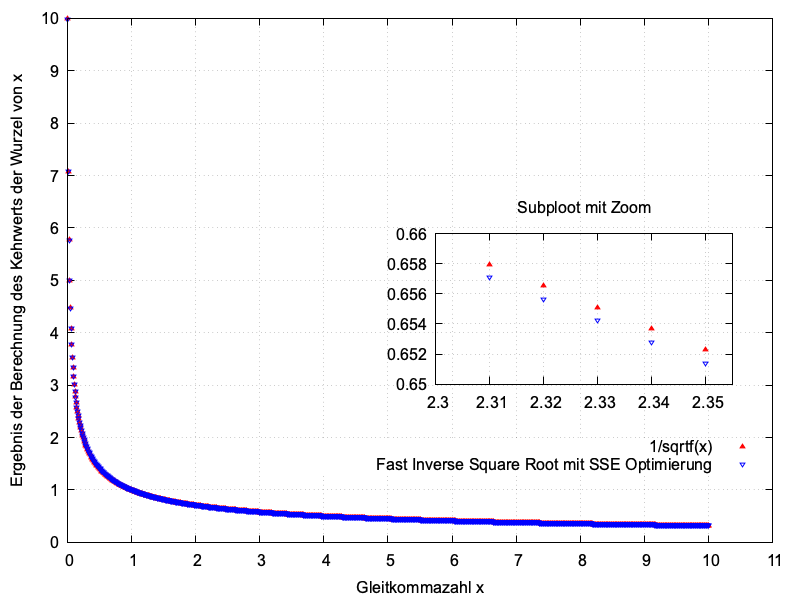
\includegraphics[width=0.8\linewidth]{images/plot_curve.png}
  \captionof{figure}{Vergleich von 1/sqrt(x) und Fast Inverse Square Root SIMD-optimiert}
  \label{fig:curve}
\end{figure}
In Abbildung 1 ist zu erkennen, dass der Algorithmus sehr nah an die exakte Berechnung herankommt und die Kurven auf den ersten Blick übereinander liegen. Wie im Subplot zu sehen ist, gibt es trotzdem kleine Abweichungen. Die Funktion aus dem originalen Sourcecode mit der MagicNumber \textbf{0x5F3759DF} hat einen maximalen relativen Fehler von $0.17522874{\%}$ \cite{Robertson}. Die Ermittlung der Genauigkeiten der optimierten MagicNumbers erfolg durch ein iteratives Verfahren. Der maximale Fehler ist unabhängig von der Größe der eingegeben Zahl, weshalb es keine bestimmten kritischen Punkte gibt, an denen der Fehler am größten ist. Demnach müssen alle möglichen Eingabewerte überprüft werden. Die berechneten Kehrwerte der Wurzeln werden verglichen mit dem exakten Ergebnis von \lstinline{1/sqrtf(x)} beziehungsweise \lstinline{1/sqrt(x)}. \par
Die Integerdarstellung aller positiven, normalisierten Floats reicht von \textbf{0x00800000} bis \textbf{0x7F800000}. Für die Überprüfung wird die Integerdarstellung bei jedem Durchlauf der Fehlerberechnung um 1 inkrementiert. Der Bereich der zu prüfenden Doubles reicht von \textbf{0x10000000000000} bis \textbf{0x7FF0000000000000}. Um alle Doubles zu überprüfen, müssten also mehr als $9*10^{18}$ Doubles überprüft werden, was zeitlich nicht machbar ist. Stattdessen wird die Integerdarstellung nach jeder Überprüfung um $1073741824$ (entspricht \lstinline{1llu << 30}) inkrementiert und es werden somit ungefähr $8.6*10^9$ Doubles überprüft. Zusätzlich zur Genauigkeit des originalen skalar-implementierten Algorithmus werden auch die Genauigkeiten des SIMD-optimierten Algorithmus sowie des skalaren Algorithmus nach zwei Newtoniterationen geprüft. Wie bereits in Kapitel 2.3 erwähnt, werden in der Implementierung die optimierten MagicNumbers von Lomont beziehungsweise Robertson verwendet. 

\begin{table}[hbt!]
\centering
\begin{tabular}{lccc}
                            & \multicolumn{3}{c}{}                                                                    \\ \cline{2-4} 
\multicolumn{1}{l|}{}       & \multicolumn{1}{c|}{\textbf{Skalar}}     & \multicolumn{1}{c|}{\textbf{Zweifache Newtoniteration}} & \multicolumn{1}{c|}{\textbf{SIMD-Optimiert}} \\ \cline{2-4} 
\multicolumn{1}{l|}{\textbf{Float}}  & \multicolumn{1}{c|}{0.1751341630} & \multicolumn{1}{c|}{0.0004792558}              & \multicolumn{1}{c|}{0.1751387360}   \\ \cline{2-4} 
\multicolumn{1}{l|}{\textbf{Double}} & \multicolumn{1}{c|}{0.1751183671} & \multicolumn{1}{c|}{0.0004597281}              & \multicolumn{1}{c|}{0.1751183671}   \\ \cline{2-4} 
\end{tabular}
\caption{Maximale relative Fehler [{\%}]}
\label{tab:captionError}
\end{table}
Auffallend ist, dass der maximale relative Fehler mit den optimierten MagicNumbers geringer ist als für die originale MagicNumber. Nach einer zusätzlichen Newtoniteration sinkt der Fehler drastisch. Der geringe Unterschied zwischen der skalaren Implementierung und der SIMD-Implementierung für Floats wird eventuell durch Präzisionsunterschiede der Instruktionen oder verschiedener Reihenfolge der Ausführung der Instruktionen hervorgerufen, da Floating-Point-Arithmetik nicht immer assoziativ ist. Der Unterschied ist jedoch unbedeutend und wird nicht weiter behandelt. \par
Insgesamt kann durch diese Untersuchung festgestellt werden, dass der Algorithmus und die verschiedenen Implementierungen davon geeignete Alternativen zur Wurzelfunktion von C darstellen und annähernde korrekte Ergebnisse für alle Floats und einen großen Bereich von Doubles liefern. Neben diesen Benchmarks werden im Programm mit der \lstinline{-t} Option außerdem kleine Tests gestartet werden. In den Tests werden für beide Implementierungen für Float und Double mit willkürlich gewählten Zahlen und Edge-Cases Ergebnisse annähernd exakt berechnet, aber da der maximale relative Fehler dies bereits bestätigt, werden sie in dieser Ausarbeitung nicht gesondert angeführt.

%=========================4. Performanzanalyse===================================
\section{Performanzanalyse}
Im Folgenden werden Benchmarks der Geschwindigkeit von verschiedenen Implementierungen des \emph{Fast Inverse Square Root} Algorithmus präsentiert. Genauer gesagt handelt es sich hierbei um Microbenchmarks, da die Geschwindigkeit von einzelnen Funktionen gemessen wird. Getestet wurde mit der gleichen Konfiguration wie in Kapitel 3.\par
Die gewählte Benchmarkmethode ist die Zeitmessung mithilfe der Funktion \emph{clock\_gettime} und der Uhr \emph{CLOCK\_MONOTONIC}. Für die Durchführung des Benchmarks werden die Berechnungen innerhalb einer Schleife öfter durchgeführt, damit die Zeit zwischen den Messungen lang genug ist. Die Messzeitpunkte sind direkt vor der Schleife und direkt nach der Schleife, somit werden fast keine für die Messung irrelevanten Instruktionen gemessen. \par
Die Korrektheit der Ergebnisse wurden durch die Überprüfung der Genauigkeit bereits sichergestellt. Weiters wurden für die Benchmarks der Intel-Turboboost und das CPU-Scaling deaktiviert, damit es zu keiner Verzerrung der Ergebnisse kommt, weil der CPU-Takt sich während des Benchmarks drastisch erhöht. Die Benchmarks wurden auf einem lokalen Rechner mit minimalen Hintergrundprozessen ausgeführt, damit die vollständigen Ressourcen zur Verfügung stehen. \par
Als Testwerte wurden 20 Arrays mit $1*10^6$ bis $10*10^6$ zufällig generierten Gleitkommazahlen genutzt. Die Berechnung der Kehrwerte der Wurzeln wurde für jedes Array mit der  C-Funktion \lstinline{1/sqrt()} und drei Varianten des Algorithmus, skalar, skalar mit 2-facher Newtoniteration und SIMD-optimiert, durchgeführt. Um mindestens eine Sekunde Abstand zwischen den Messungen sicherzustellen und Störungen zu dämpfen, wurde jede Berechnung einer Implementierung 200 mal durchgeführt. Anschließend wurde die mittlere Laufzeit jeder Implementierung gebildet. Die Ergebnisse sind in den folgenden Grafiken und Tabellen zu sehen.
\begin{figure}[H]
\centering
  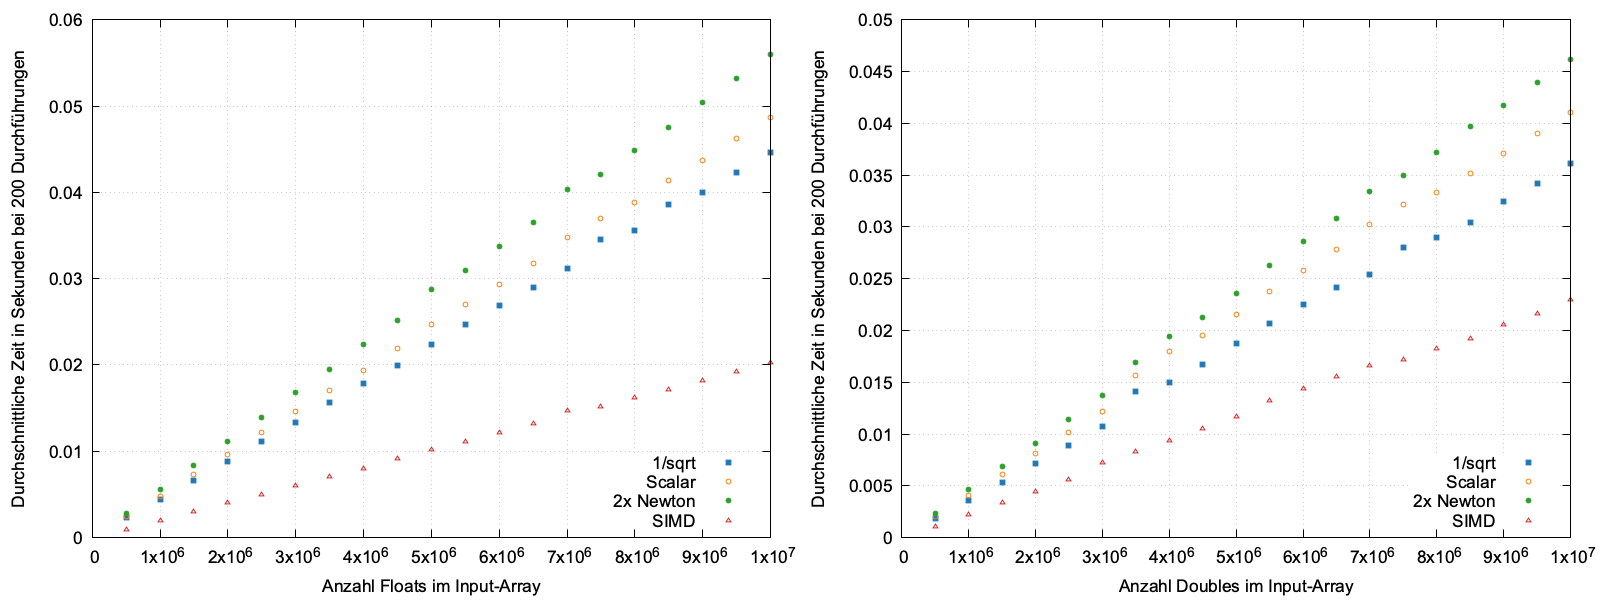
\includegraphics[width=1.0\linewidth]{images/plot_speed.png}
  \captionof{figure}{Laufzeit der Implementierungen für Float (l) und Double (r)}
  \label{fig:runtime}
\end{figure}
%Zwei Tabellen mit Zeitverhältnis zu 1/sqrt(x)
\begin{table}[hbt!]
\centering
\begin{tabular}{l|c|c|c|}
\cline{2-4}
                & \textbf{Skalar} & \textbf{Zweifache Newtoniteration} & \textbf{SIMD-Optimiert} \\ \cline{2-4} 
\textbf{Float}  & 0.9181            & 0.7980                             & 2.2097                  \\ \cline{2-4} 
\textbf{Double} & 0.8731            & 0.7835                             & 1.5871                  \\ \cline{2-4} 
\end{tabular}
\caption{Durchschnittliches Laufzeitverhältnis von \lstinline{1/sqrt()} zu Implementierungen}
\label{tab:captionRuntime}
\end{table}
Die Zeitverläufe sind annähernd linear mit Ausnahme von kleinen Abweichungen, was darauf hindeutet, dass die Berechnungen nicht wegoptimiert wurden. Wie zu erwarten war, bringt die zweifache Newtoniteration eine etwas schlechtere Performanz mit sich. Die SIMD-Implentierungen für Floats und Doubles haben jeweils einem Speedup-Faktor von 2.406 und 1.818 zu ihren skalaren Gegenstücken. Auch, wenn für die SIMD-Implementierung für Floats eine höhere Beschleunigung erwartet wurde, bieten beide Faktoren eine bedeutungsvolle Steigerung der Recheneffizienz. \par 
Verwunderlich ist jedoch, dass die Berechnung mit \lstinline{1/sqrt()} schneller ist als mit dem \emph{Fast Inverse Square Root} Algorithmus. Wirft man auf den Blick des generierten Assembler Codes wird sichtbar, dass der GCC-Compiler \lstinline{1/sqrt()} mit den SSE-Instruktionen \lstinline{_mm_div_ss/ds und _mm_sqrt_ss/ds} ersetzt. Wird zusätzlich mit der Flag \lstinline{-ffast-math} kompiliert, wird die Berechnung sogar durch \lstinline{_mm_rsqrt_ss/sd} ersetzt. Diese Instruktionen für die Division und Wurzelberechnung wurden mit der Intel-SSE Extension veröffentlicht, basieren auf Hardware und liefern daher schnellere Berechnungszeiten, was den Geschwindigkeitsunterschied erklärt.

\section{Zusammenfassung und Ausblick}
Diese Ausarbeitung bietet einen Einblick in die Funktionsweise des \emph{Fast Inverse Square Root} und präsentiert eine SIMD-optimierte Version Implementierung, auch erweitert für die Berechnung mit Doubles. Die wichtigsten Schritte und die mathematischen Grundlagen hinter dem Algorithmus und der MagicNumber wurden erläutert, wodurch die bemerkenswerte Kombination von Bithacking und numerischer Annäherung zur Geltung kommt. Durch einen \emph{Brute-Force-}Ansatz wurde die MagicNumber für Floats \boldmath $R = \textbf{0x5F375A87}$ \unboldmath und für Doubles \boldmath$R_d = \textbf{ 0x5FE6EB50C7B33600}$ \unboldmath ermittelt, die auch eine hohe Genauigkeit liefern und nah an die bereits etablierten MagicNumbers von Lomont und Robertson kommen. Die Genauigkeit und Performanz des Algorithmus im Vergleich zu alternativen Berechnungen wurden durch wissenschaftliche Verfahren erfasst und die Ergebnisse wurden diskutiert. Dabei wurde festgestellt, dass heutige Prozessoren und Compiler dem Algorithmus durch Optimierung und Verwendung von SSE-Instruktionen wie \lstinline{rsqrtss} oder sogar AVX-Instruktionen wie \lstinline{vrsqrtss} überlegen sind, der Algorithmus aber für damalige Zeiten eine außerordentlich gute Annäherung mit einer bedeutend schnelleren Berechnungszeit liefern konnte. Weitere Optimierungsmöglichkeiten bestehen darin, die AVX-Extension zu nutzen und somit mehr als 4 Floats beziehungsweise 2 Doubles gleichzeitig zu verarbeiten und die resultierenden Konstanten der Newtoniteration und MagicNumber mit 3D-Optimierung zu verbessern, um noch genauere Ergebnisse zu erzielen \cite{kadlec}.
% TODO: Fuegen Sie Ihre Quellen der Datei Ausarbeitung.bib hinzu
% Referenzieren Sie diese dann mit \cite{}.
\newpage
\bibliographystyle{unsrt}
\bibliography{Ausarbeitung}{}

\end{document}